The \Muujj distributions of simulated leptoquark samples in each year of data-taking are shown in Figs.~\ref{figapp:lqsim1} and~\ref{figapp:lqsim2}. Samples are the same MC samples used in the rest of the analysis, described in Section~\ref{sec:SimSignal}. Each sample has the preselection, MC corrections, and b tag requirements applied, and is normalized to the product of the signal cross section and integrated luminosity in each data-taking year. 

\begin{figure}[H]
    \centering
    {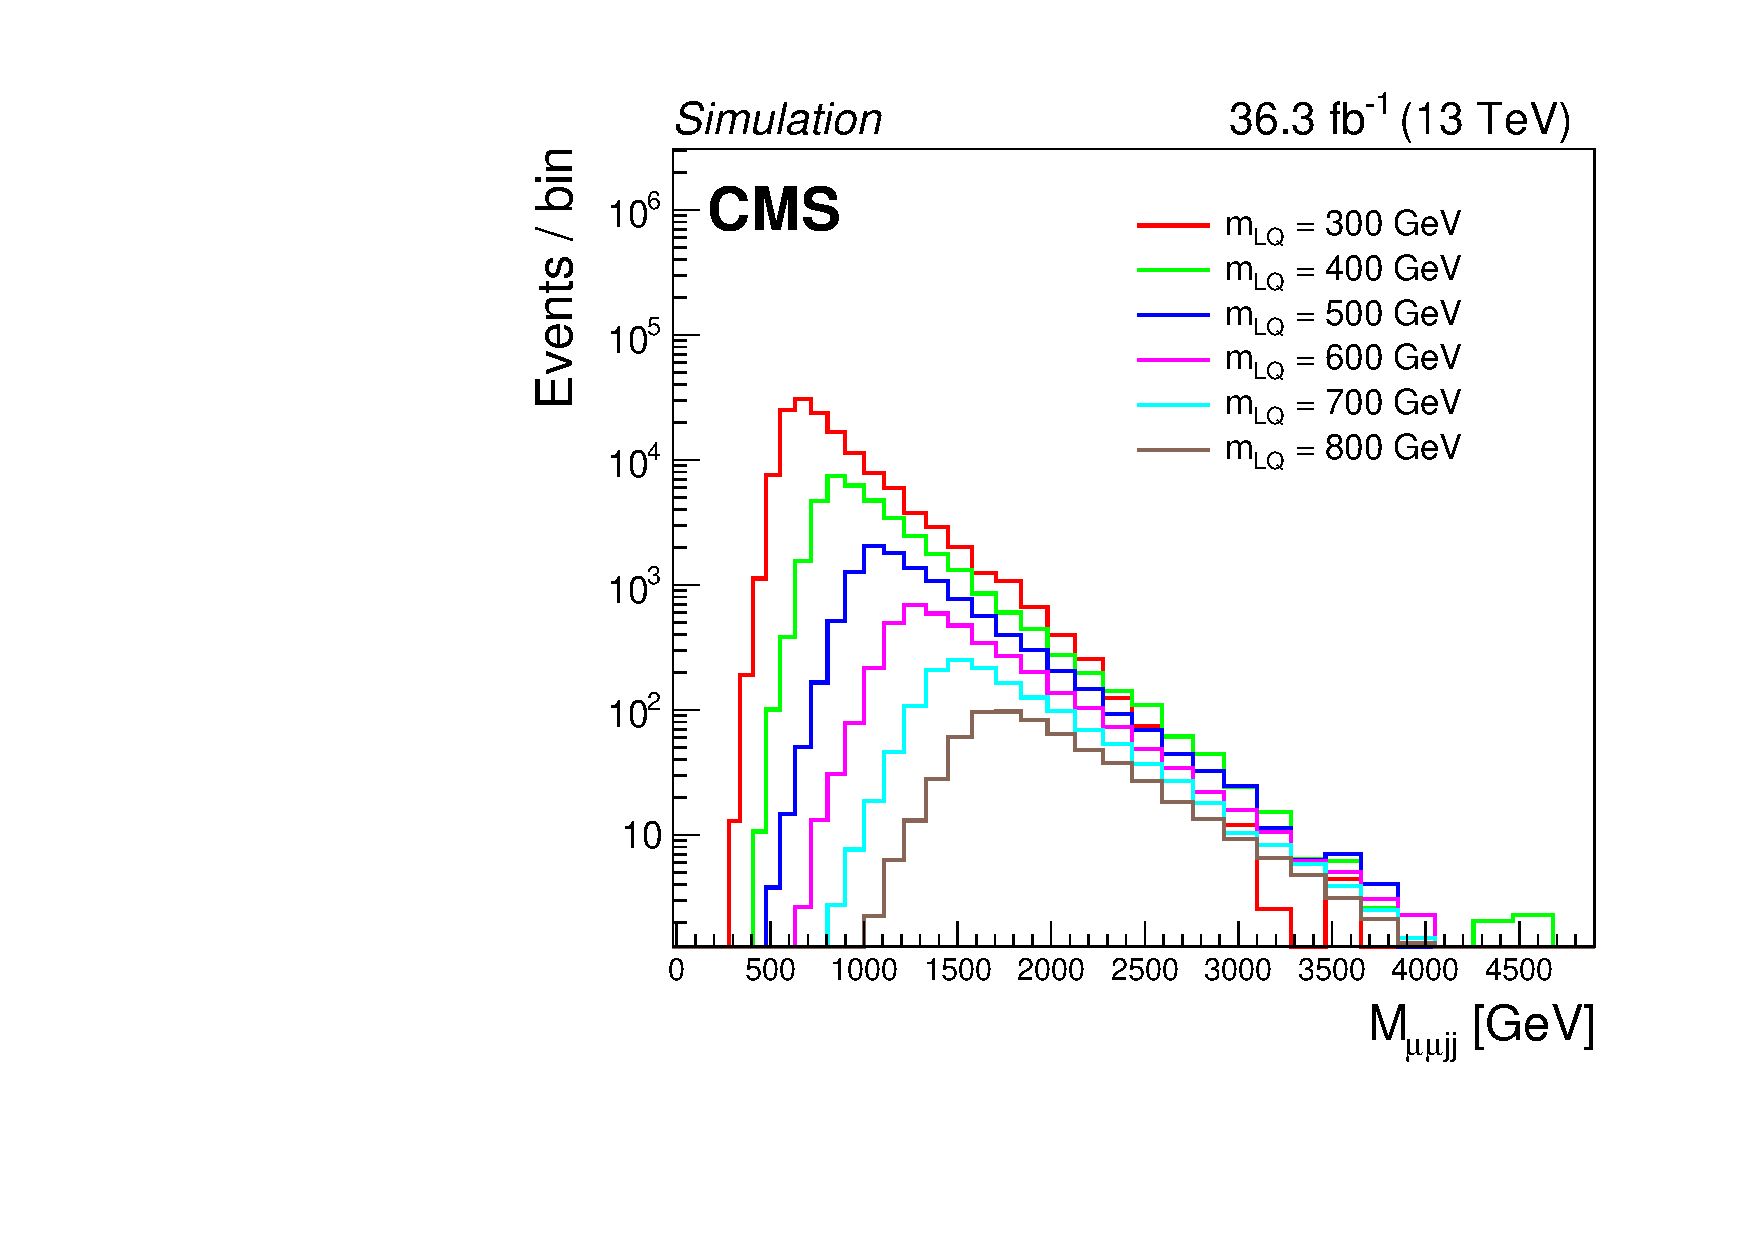
\includegraphics[width=.32\textwidth]{Images/Analysis/SignalMassStudy/2016/Mujbj_M300_to_M800.pdf}}
    {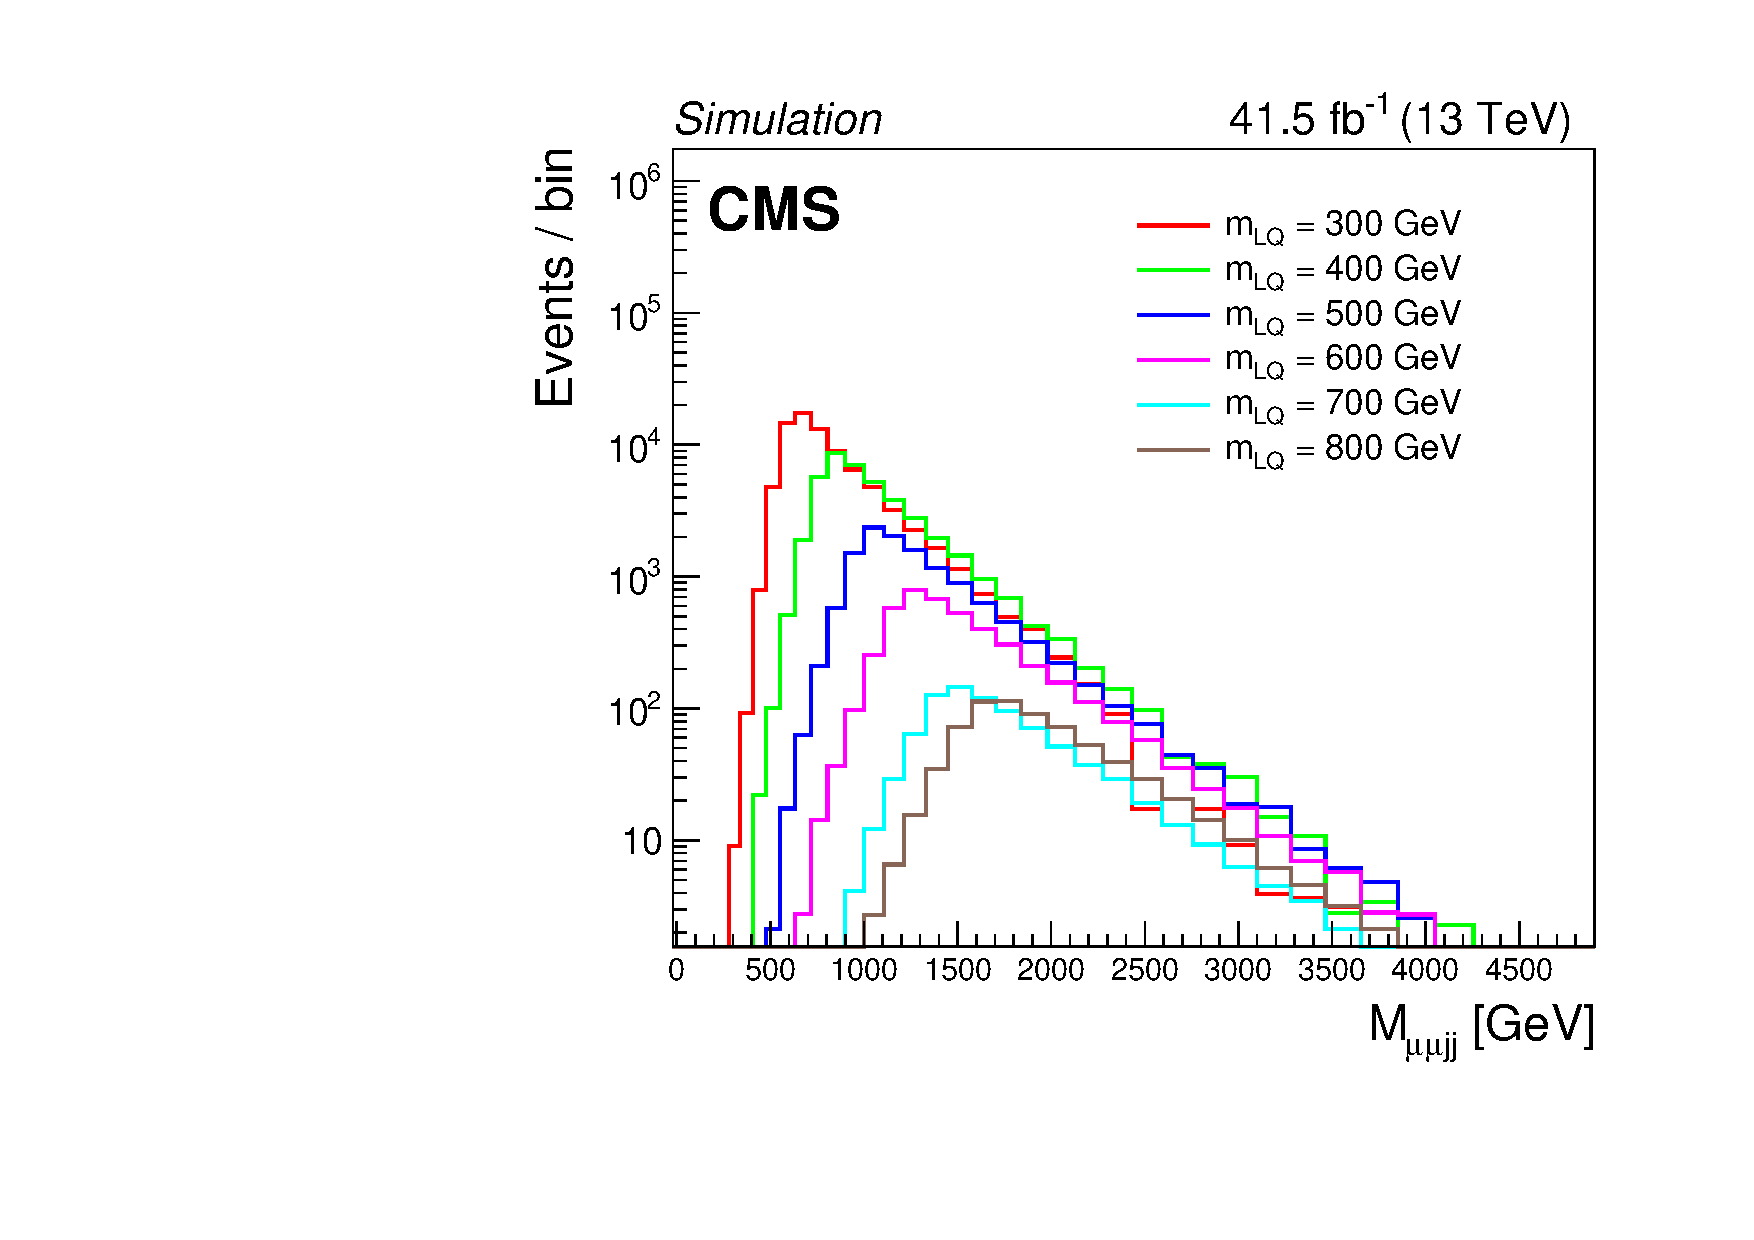
\includegraphics[width=.32\textwidth]{Images/Analysis/SignalMassStudy/2017/Mujbj_M300_to_M800.pdf}}
    {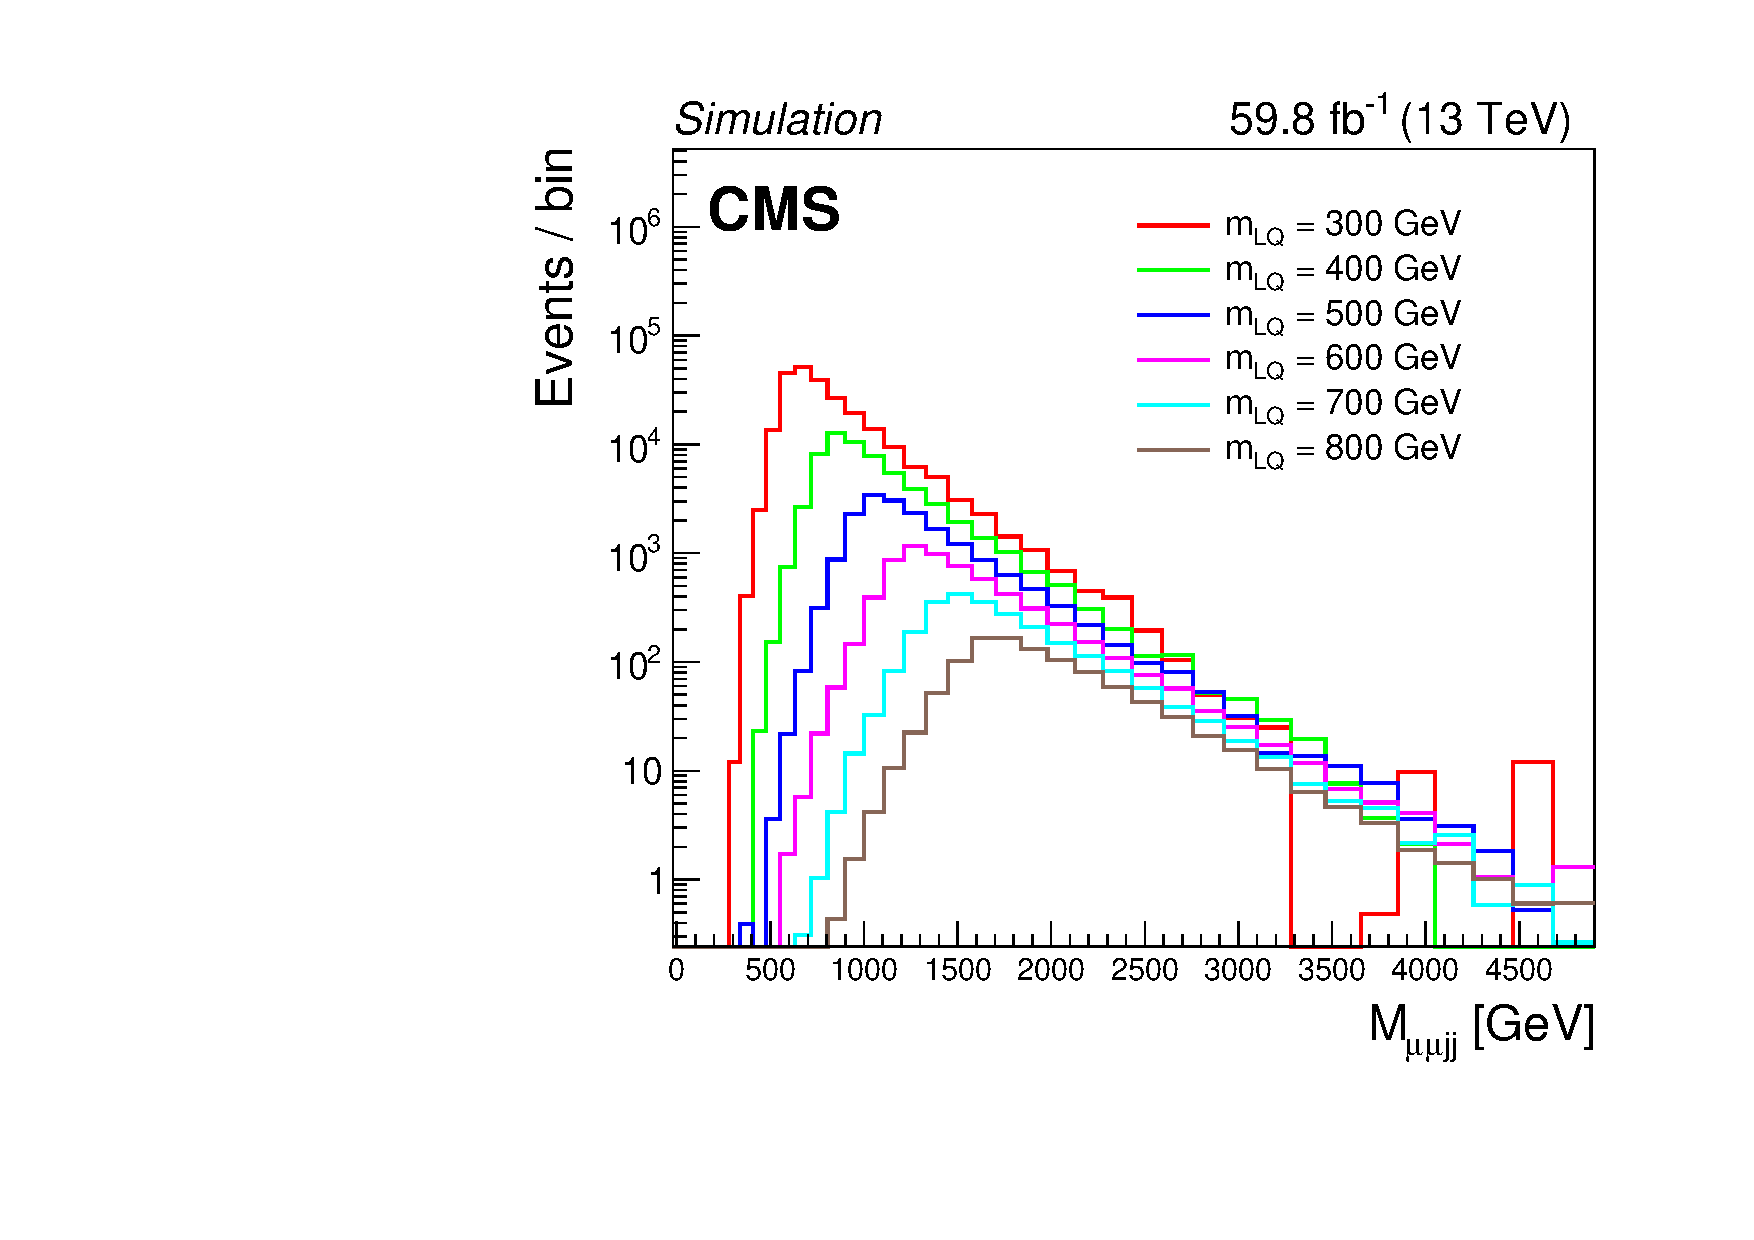
\includegraphics[width=.32\textwidth]{Images/Analysis/SignalMassStudy/2018/Mujbj_M300_to_M800.pdf}}
    {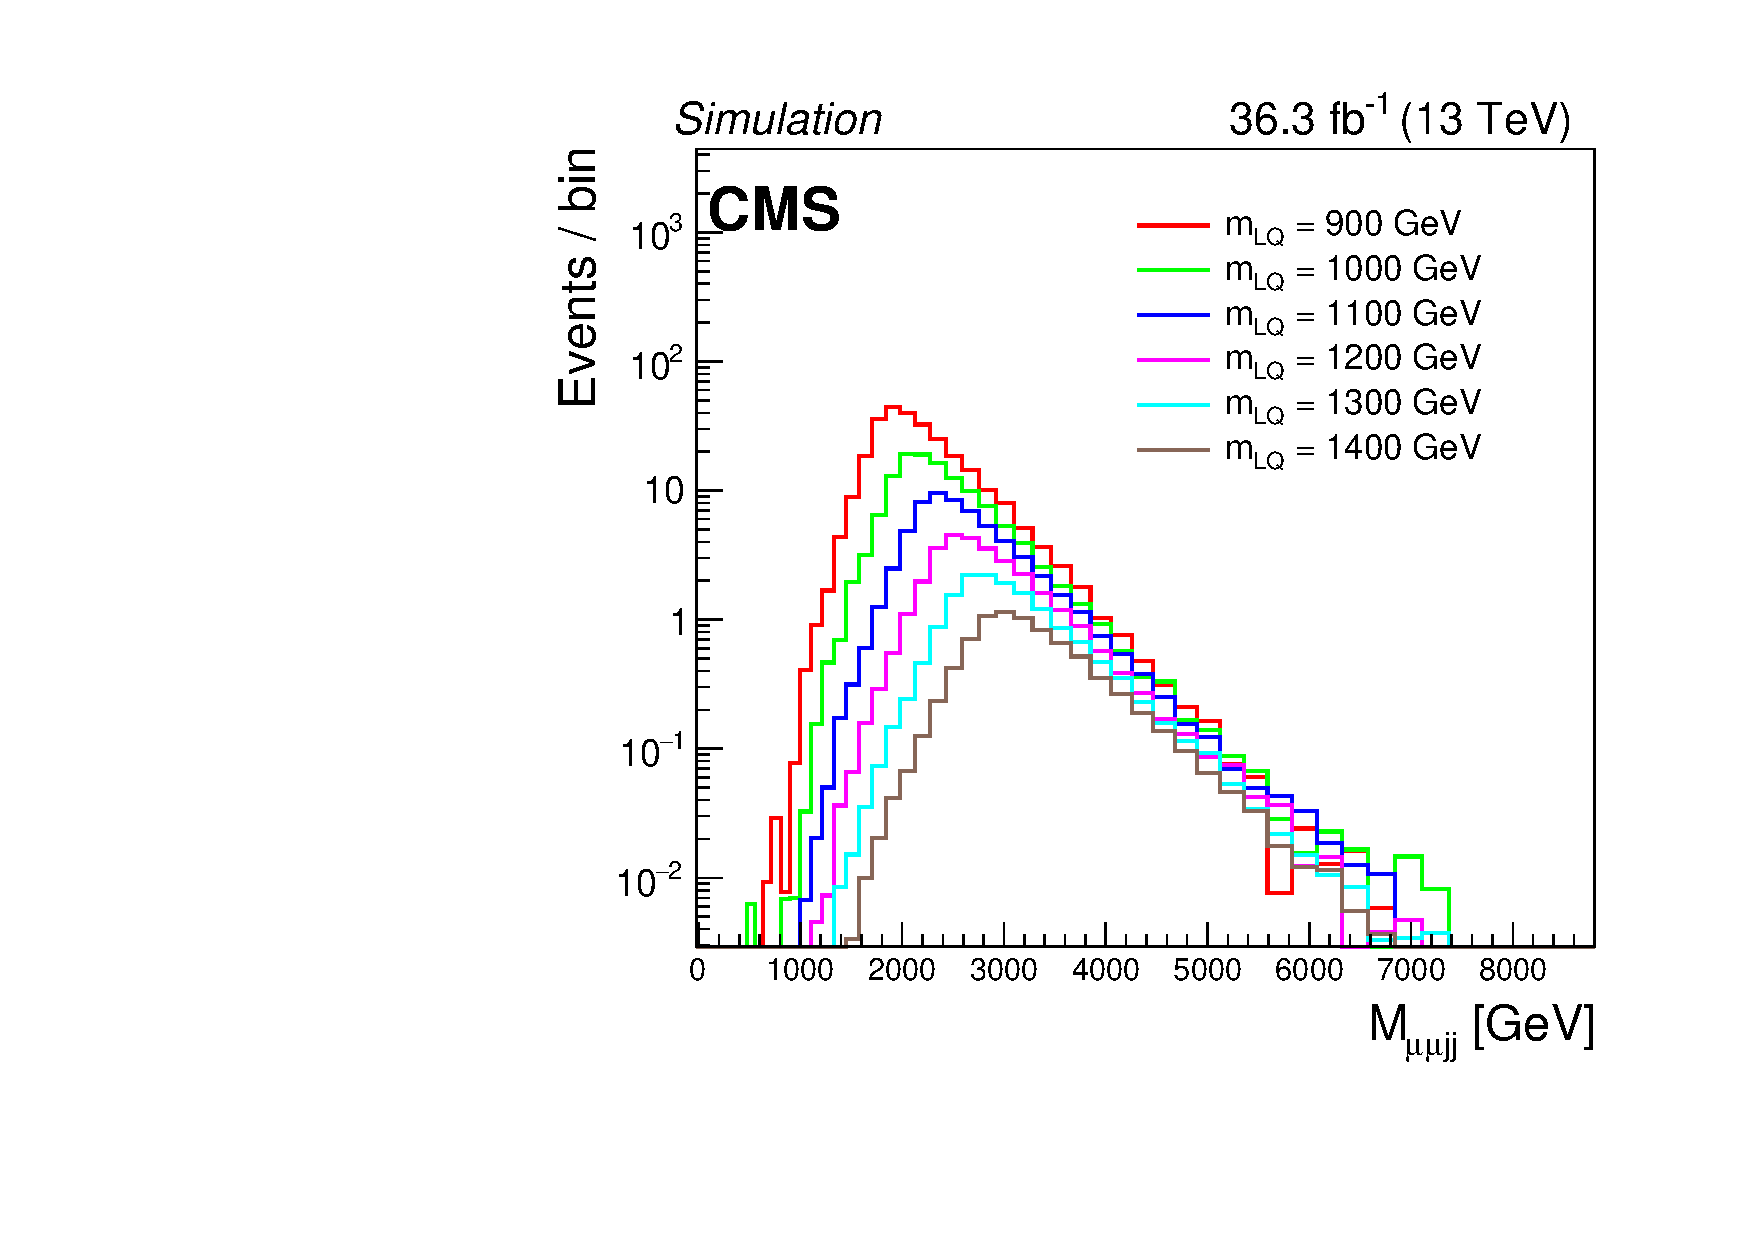
\includegraphics[width=.32\textwidth]{Images/Analysis/SignalMassStudy/2016/Mujbj_M900_to_M1400.pdf}}
    {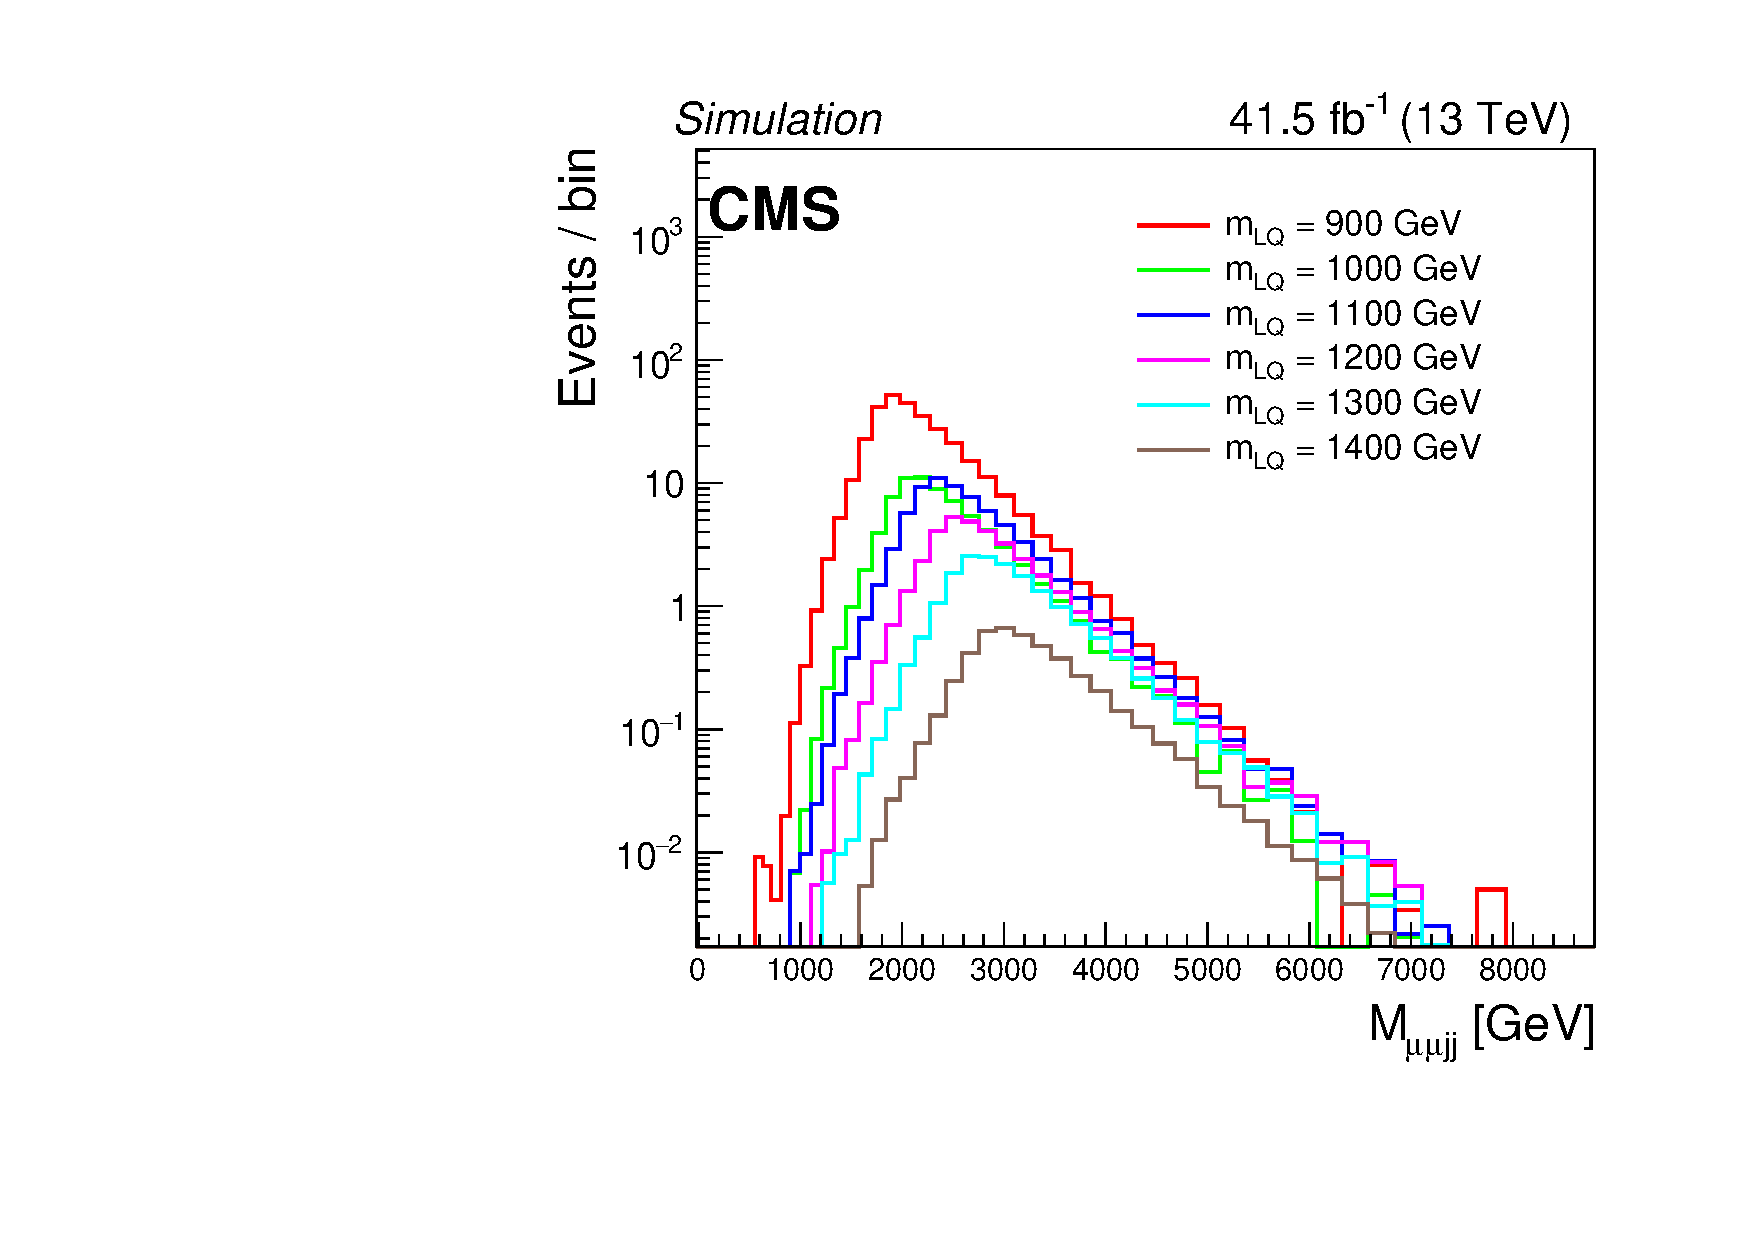
\includegraphics[width=.32\textwidth]{Images/Analysis/SignalMassStudy/2017/Mujbj_M900_to_M1400.pdf}}
    {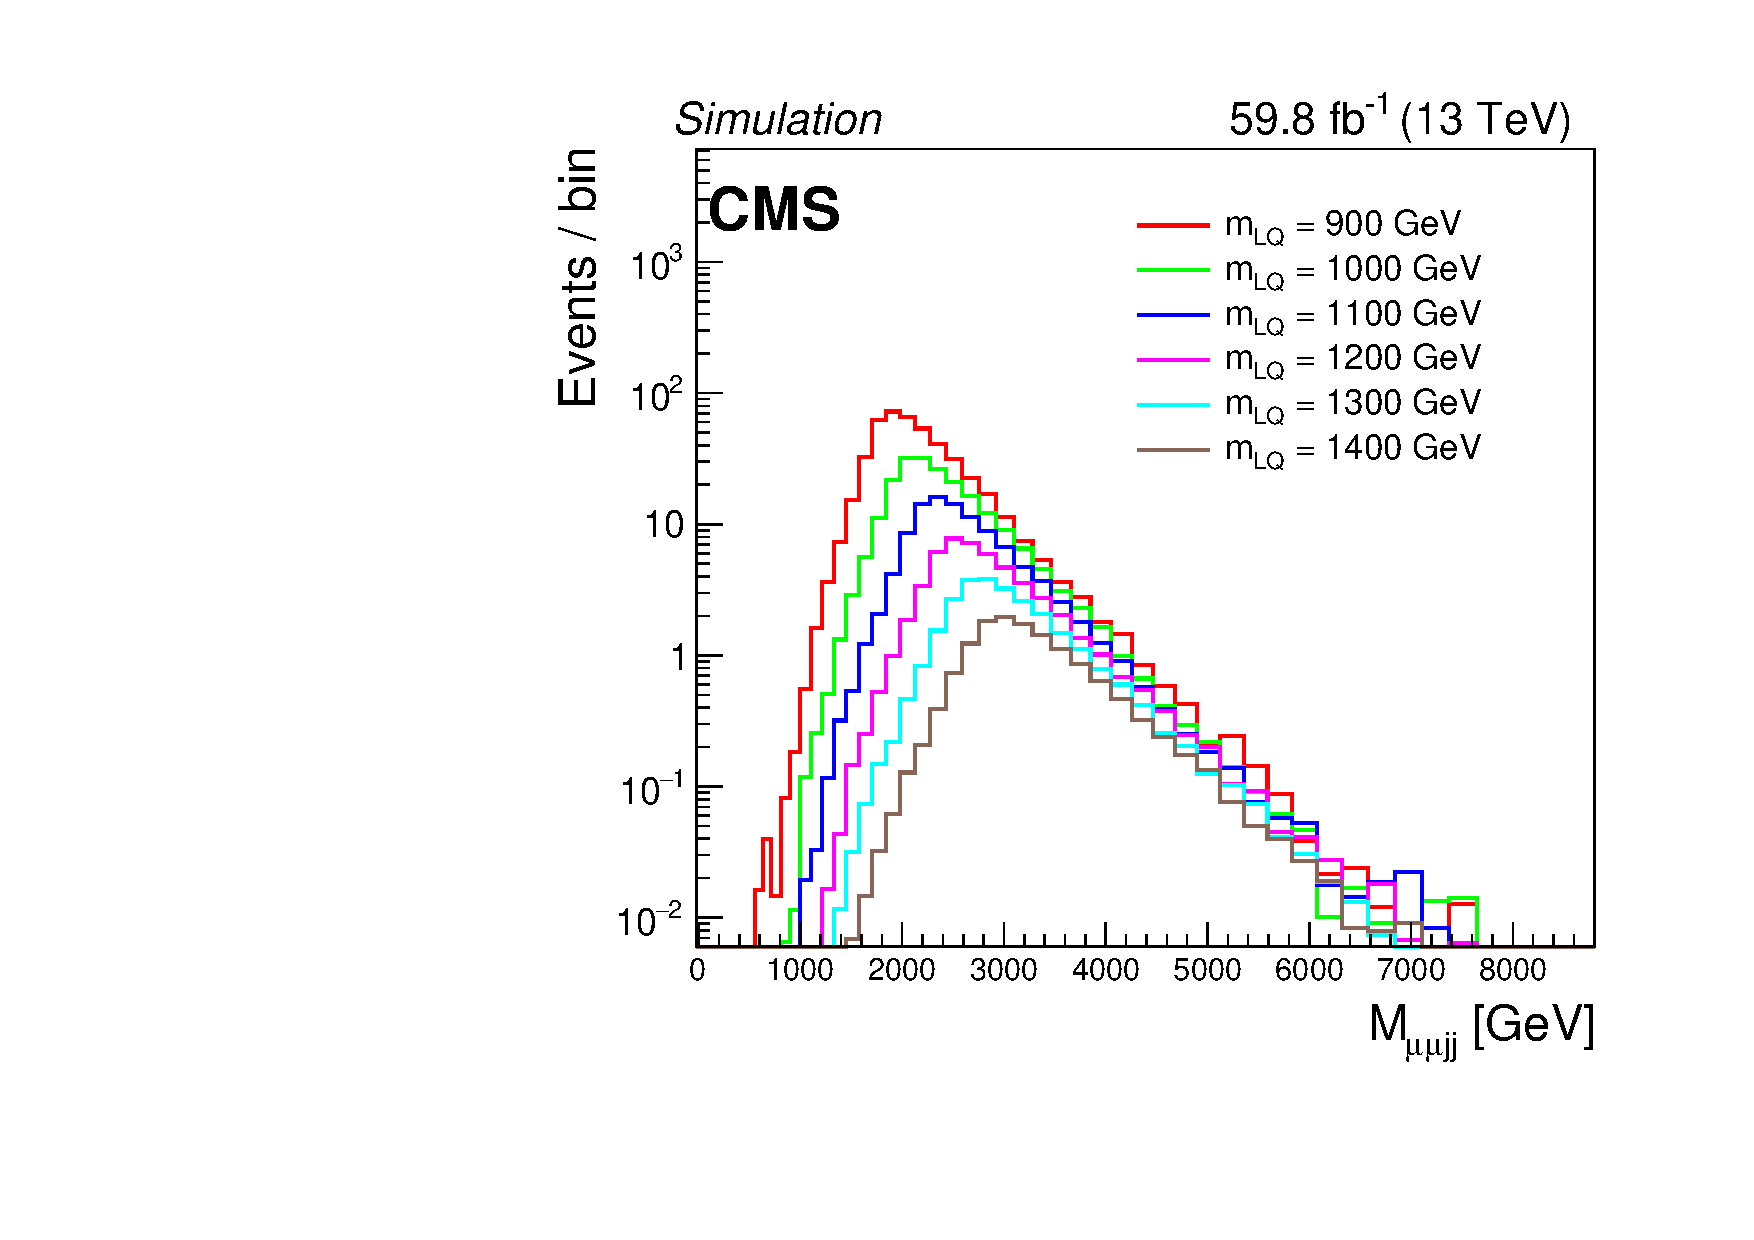
\includegraphics[width=.32\textwidth]{Images/Analysis/SignalMassStudy/2018/Mujbj_M900_to_M1400.pdf}}
    {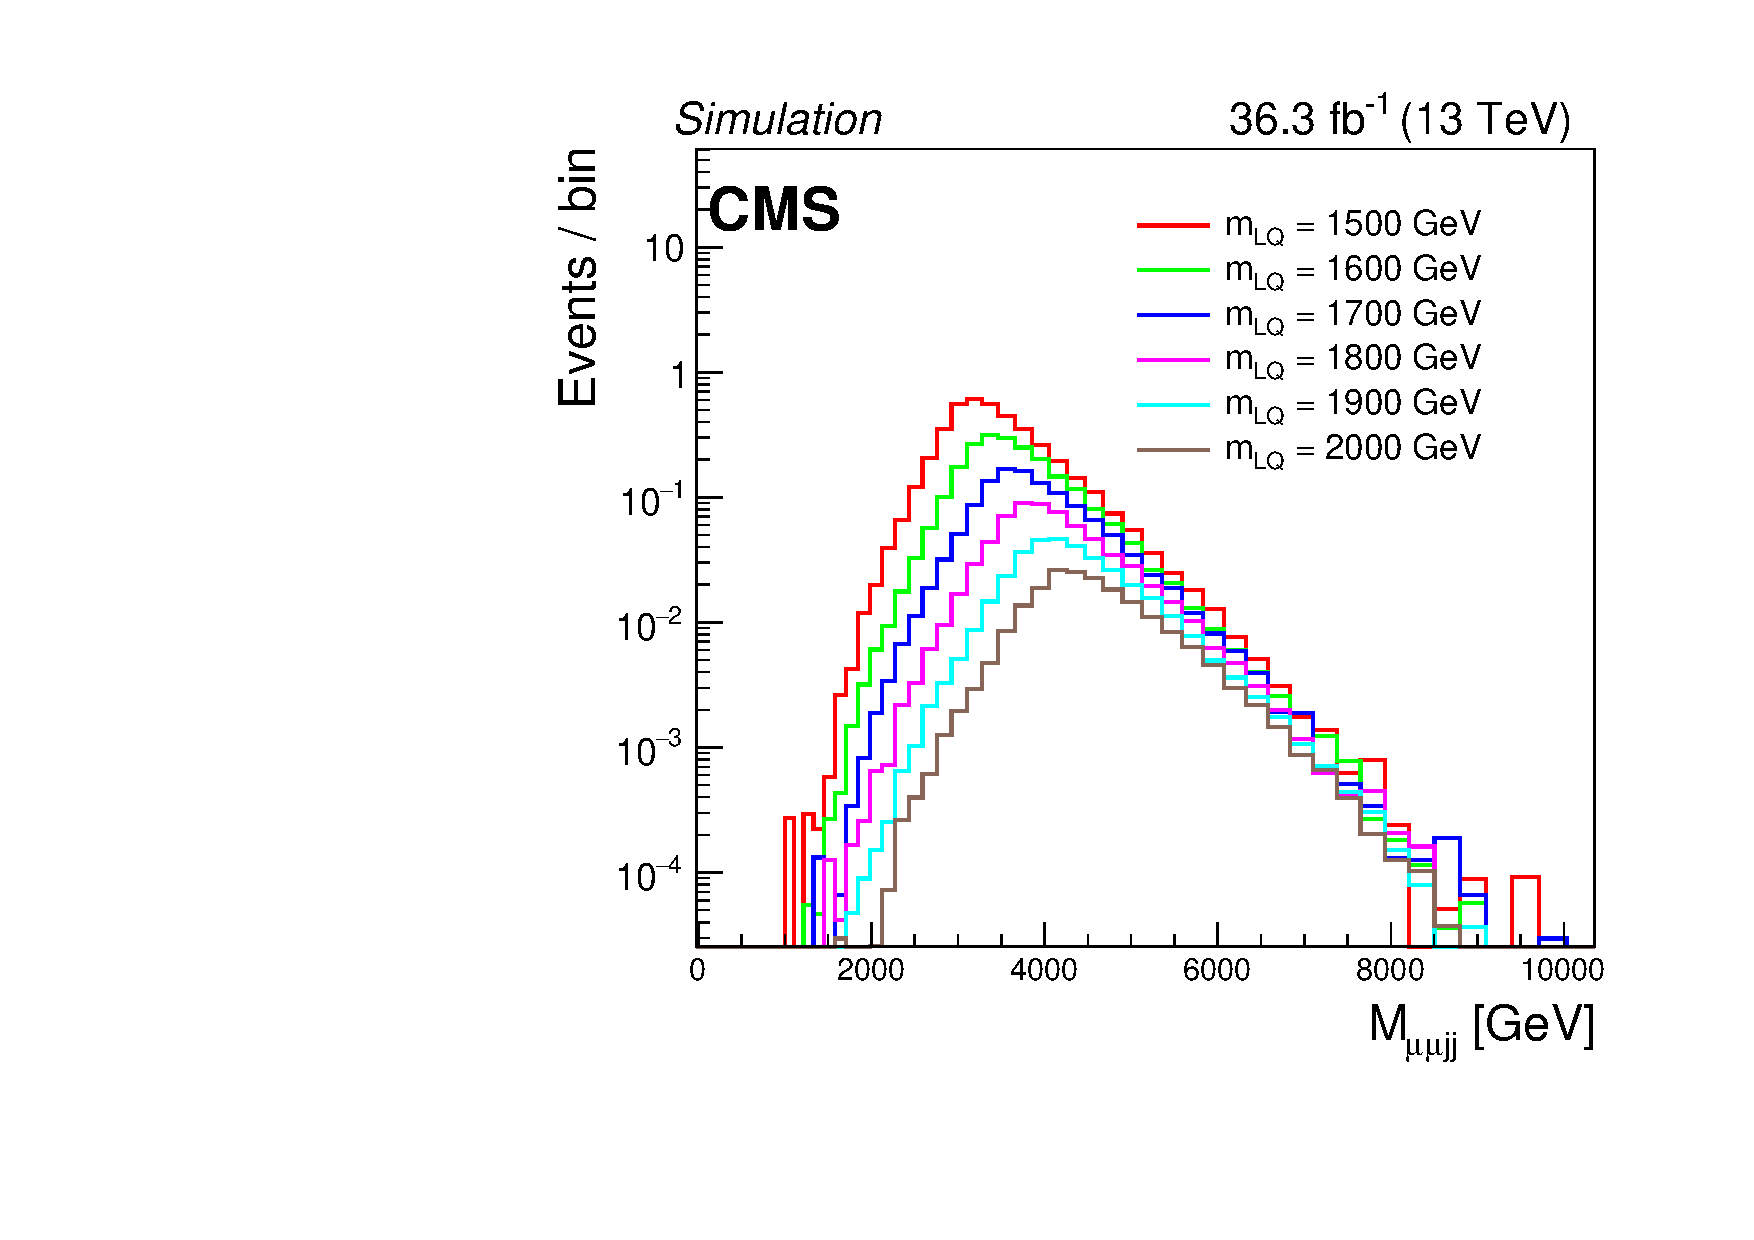
\includegraphics[width=.32\textwidth]{Images/Analysis/SignalMassStudy/2016/Mujbj_M1500_to_M2000.pdf}}
    {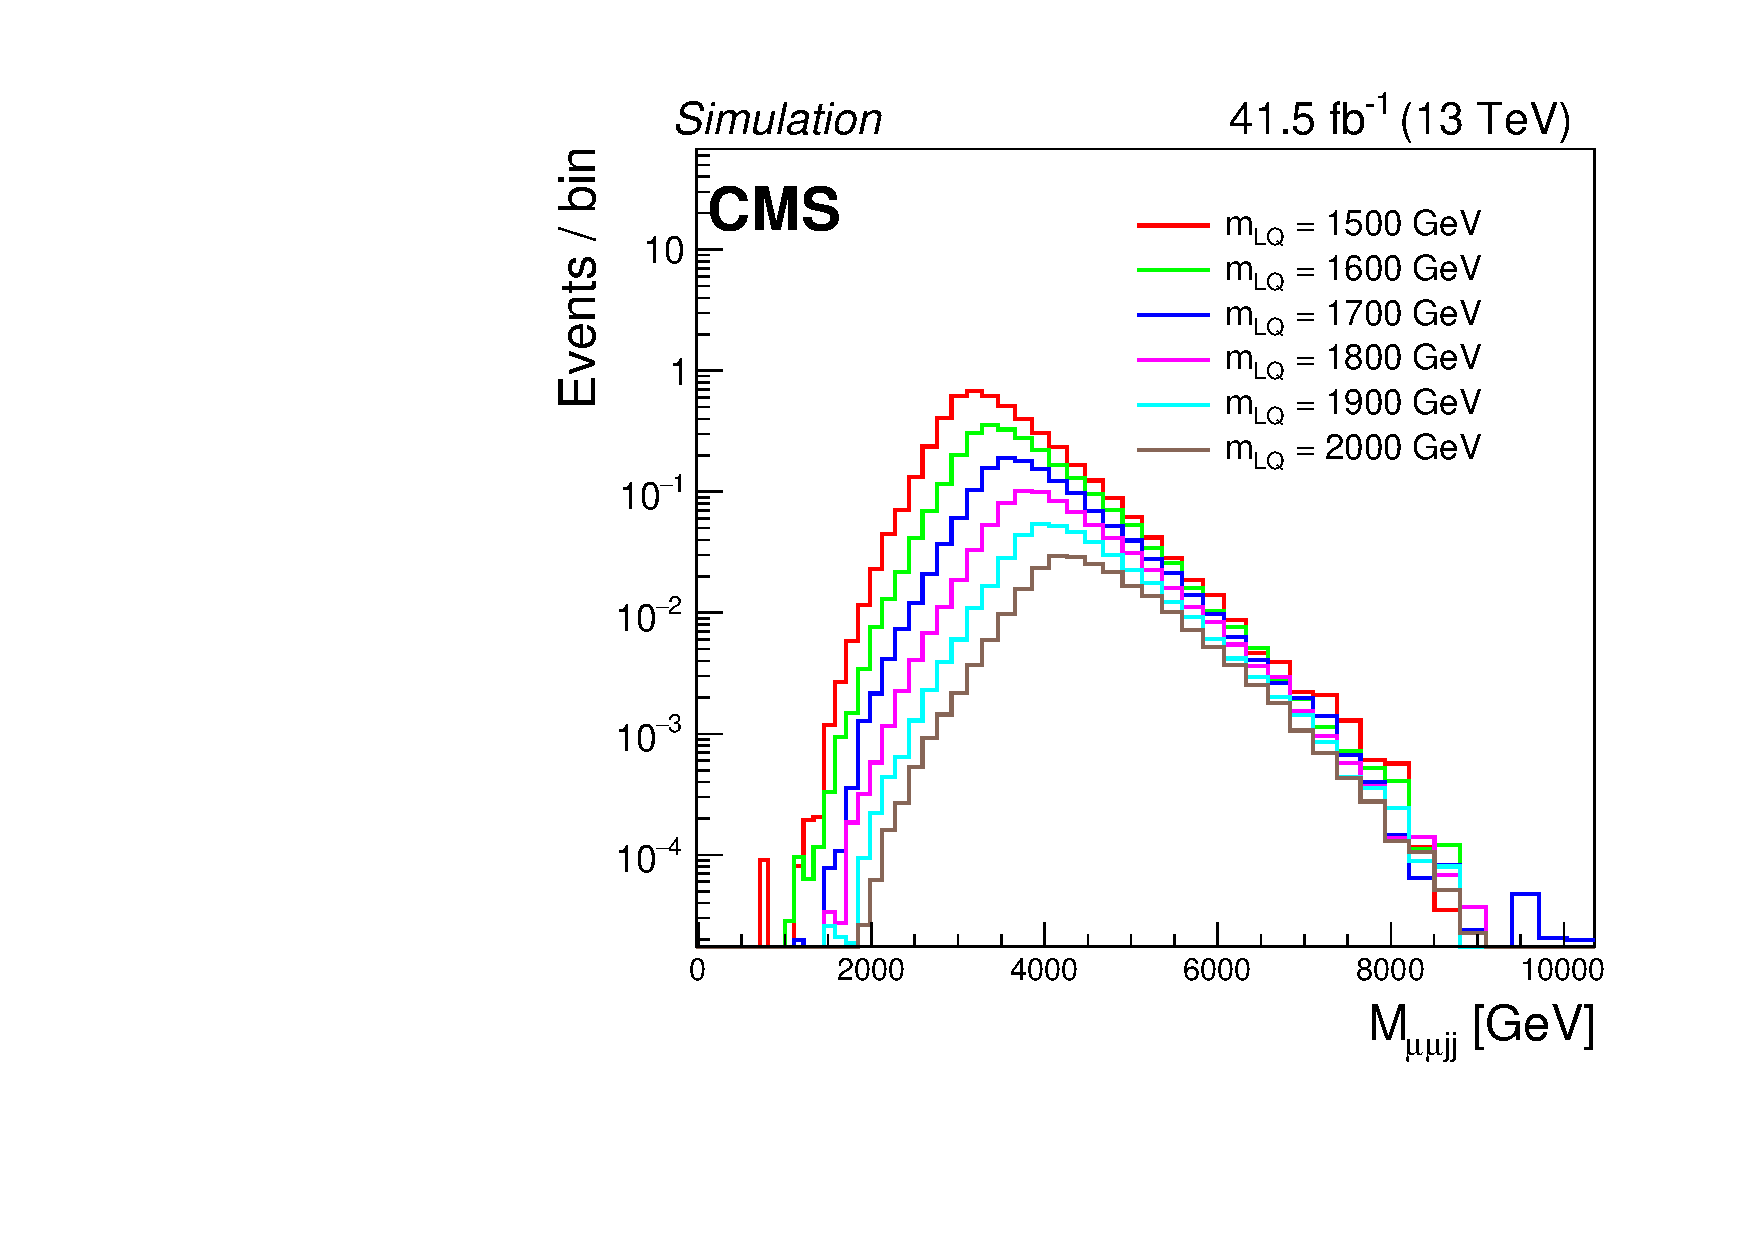
\includegraphics[width=.32\textwidth]{Images/Analysis/SignalMassStudy/2017/Mujbj_M1500_to_M2000.pdf}}
    {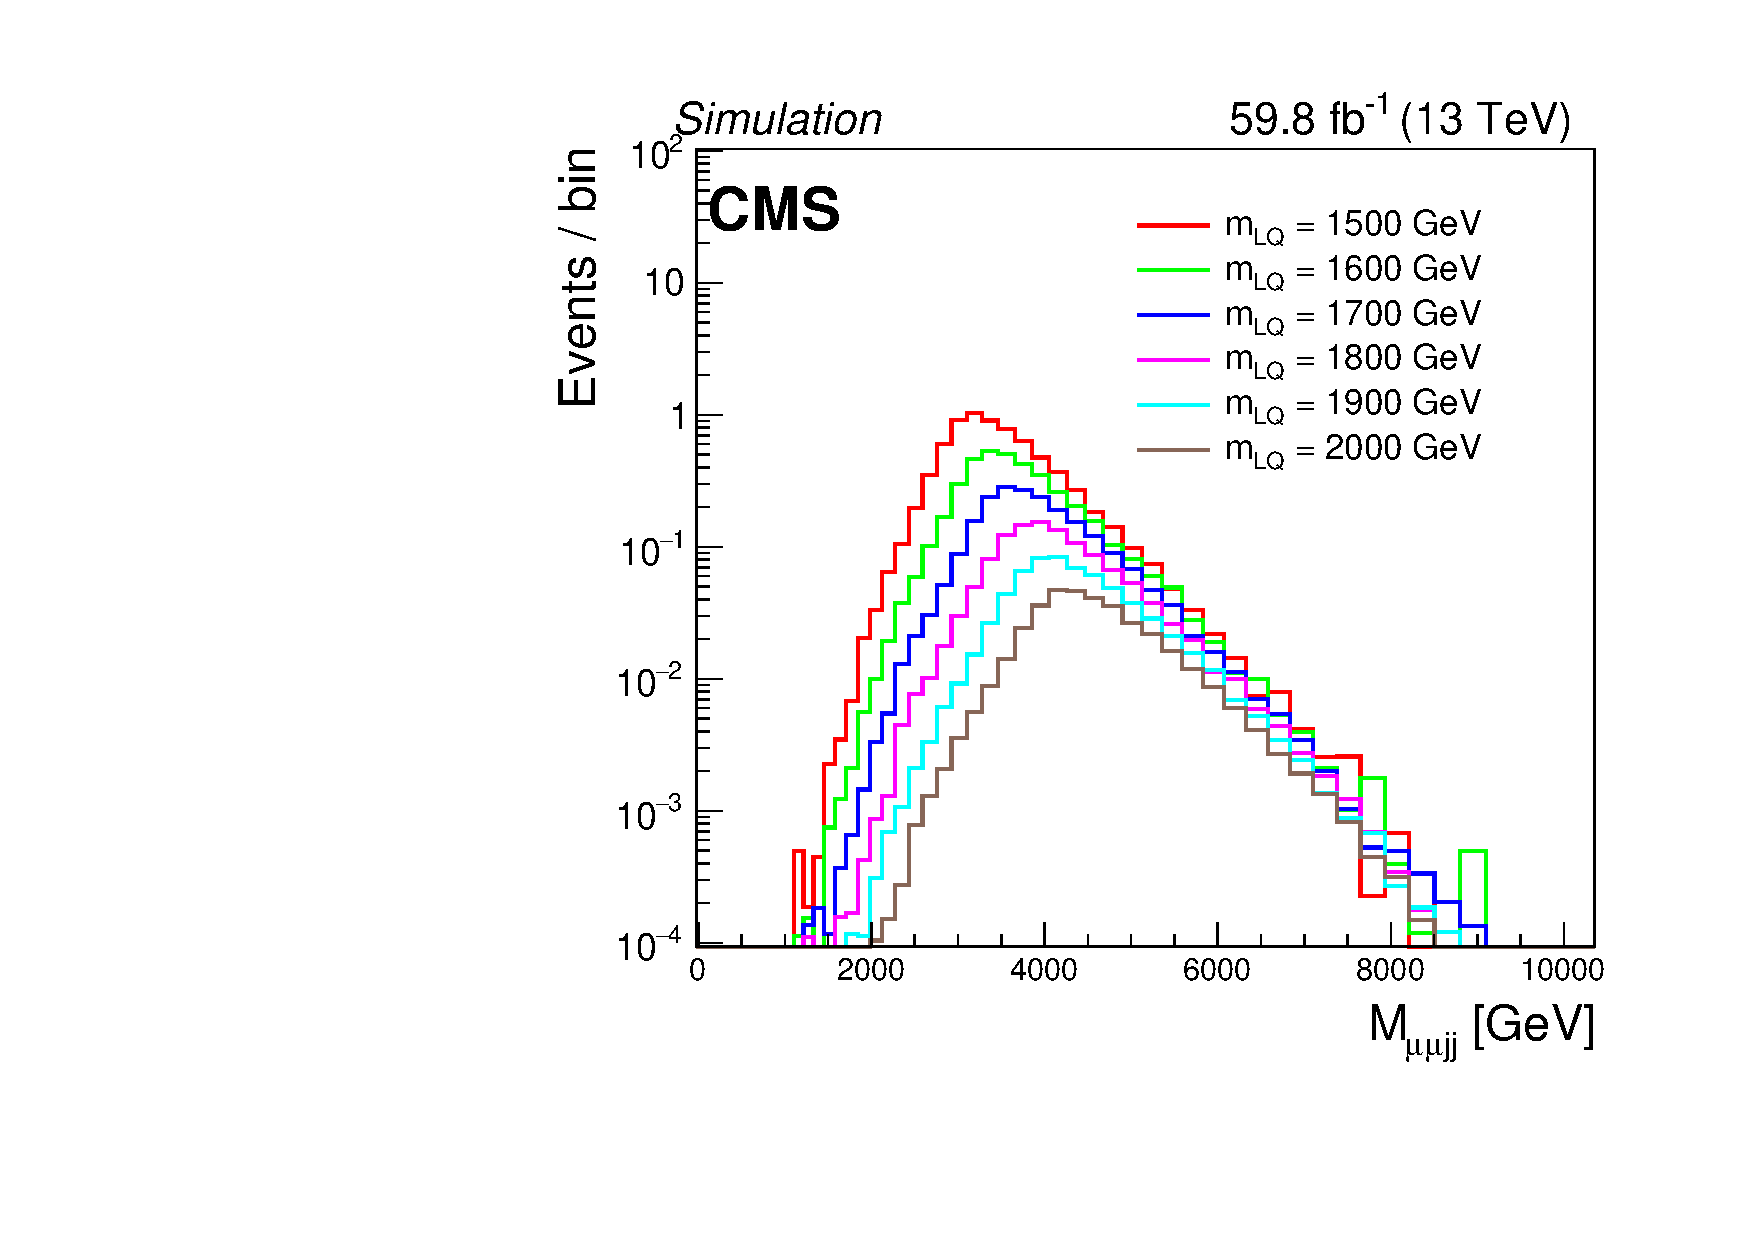
\includegraphics[width=.32\textwidth]{Images/Analysis/SignalMassStudy/2018/Mujbj_M1500_to_M2000.pdf}}
    \caption{The preselection-level \Muujj distributions of simulated leptoquark pair samples for the data-taking periods 2016 (left), 2017 (middle), and 2018 (right). For clarity, each plot overlays the distributions corresponding to a set of six leptoquark masses: \SI{300}{} to \SI{800}{GeV} (top), \SI{900}{} to \SI{1400}{GeV} (middle), and \SI{1500} to \SI{2000}{GeV} (bottom).}
    \label{figapp:lqsim1}
\end{figure}

\begin{figure}[H]
    \centering
    {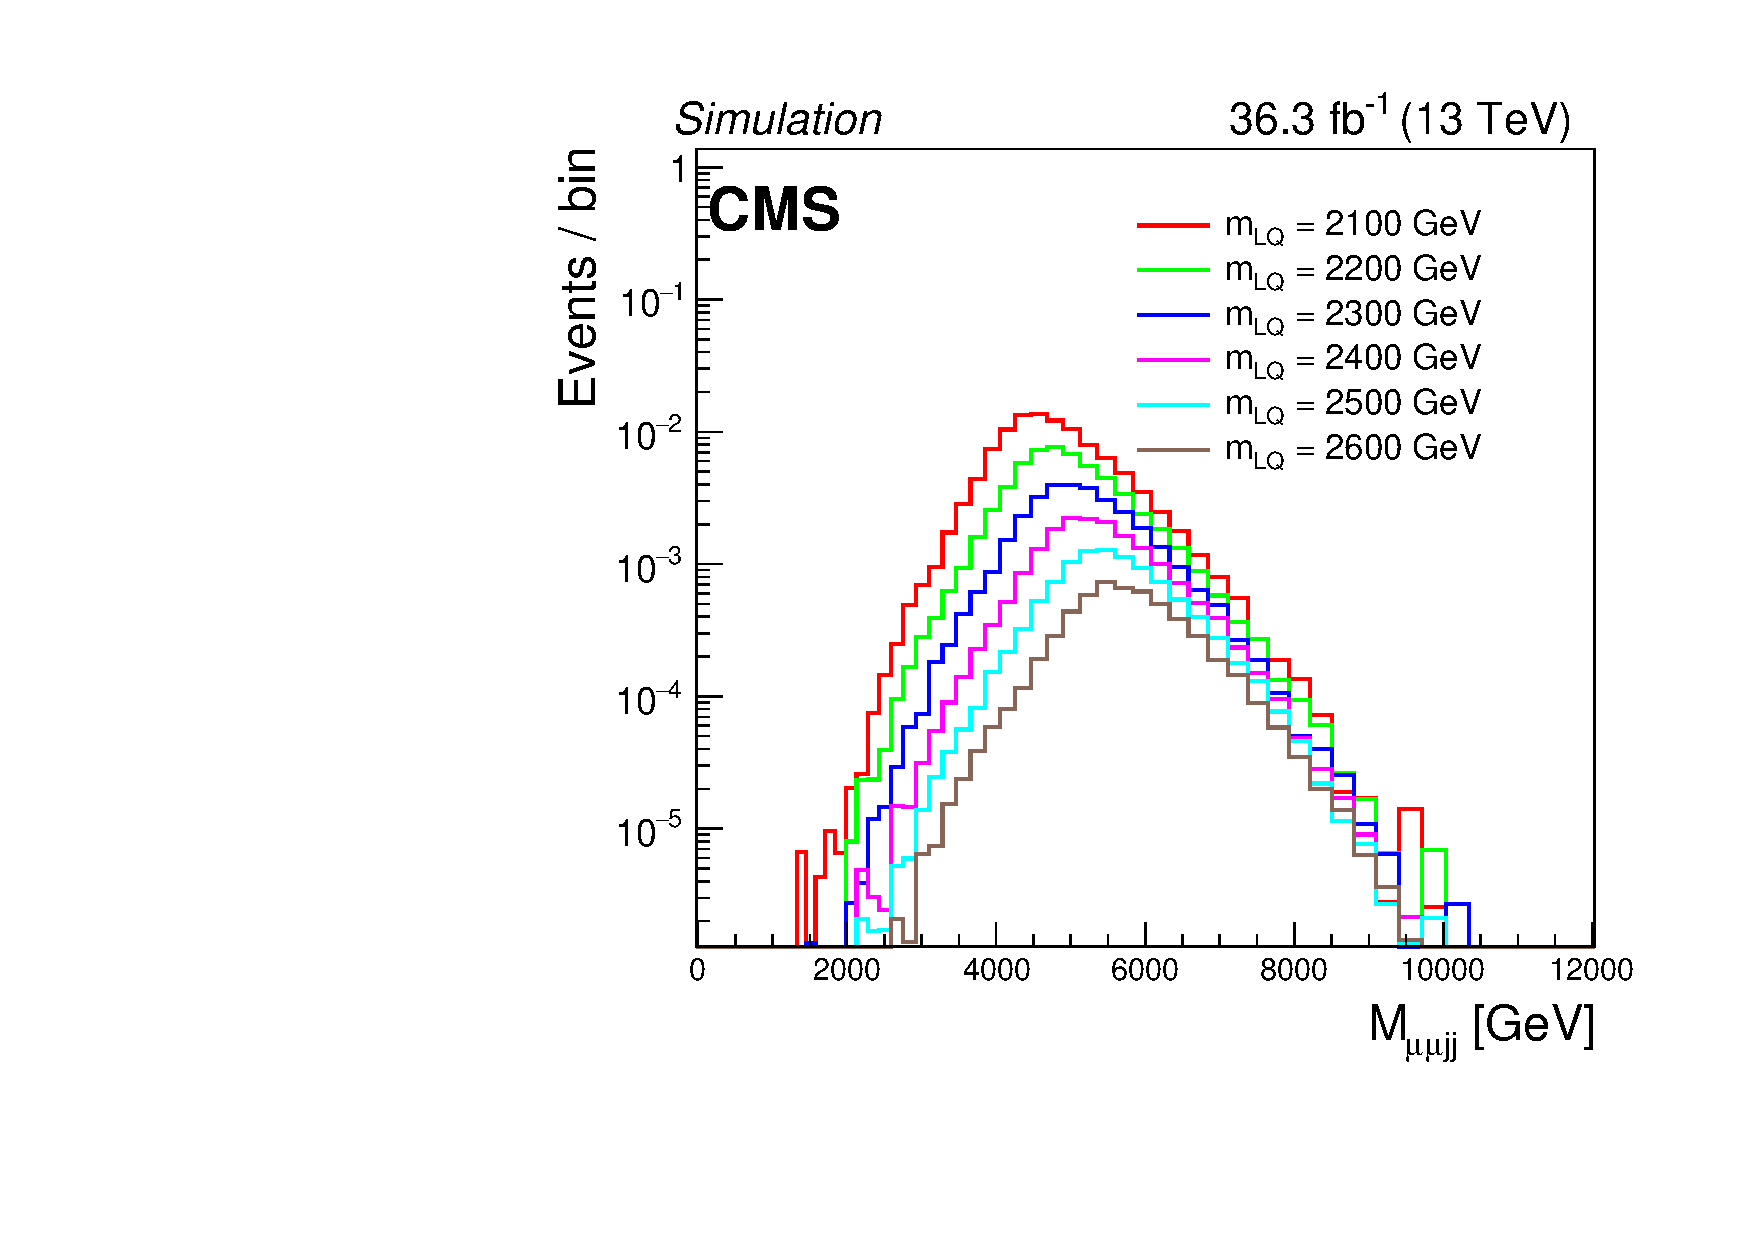
\includegraphics[width=.32\textwidth]{Images/Analysis/SignalMassStudy/2016/Mujbj_M2100_to_M2600.pdf}}
    {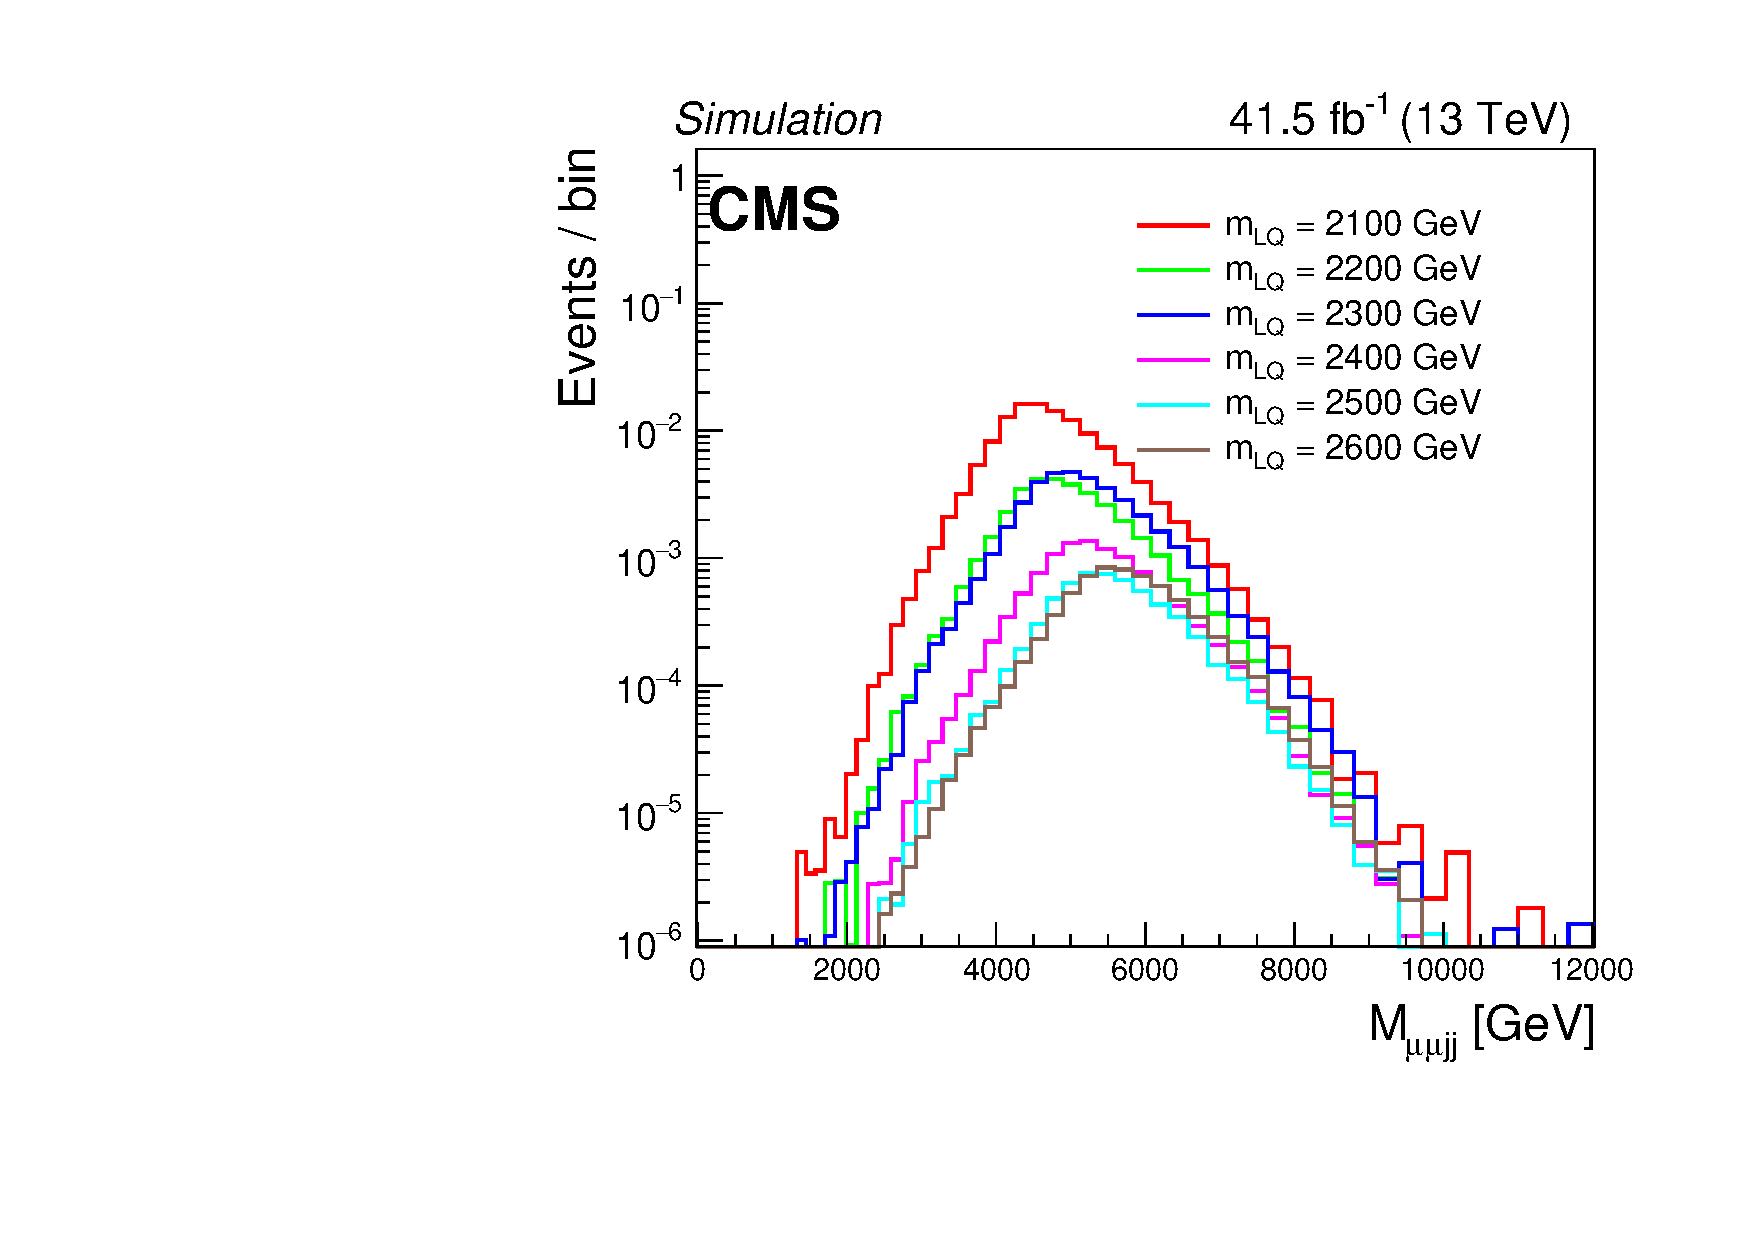
\includegraphics[width=.32\textwidth]{Images/Analysis/SignalMassStudy/2017/Mujbj_M2100_to_M2600.pdf}}
    {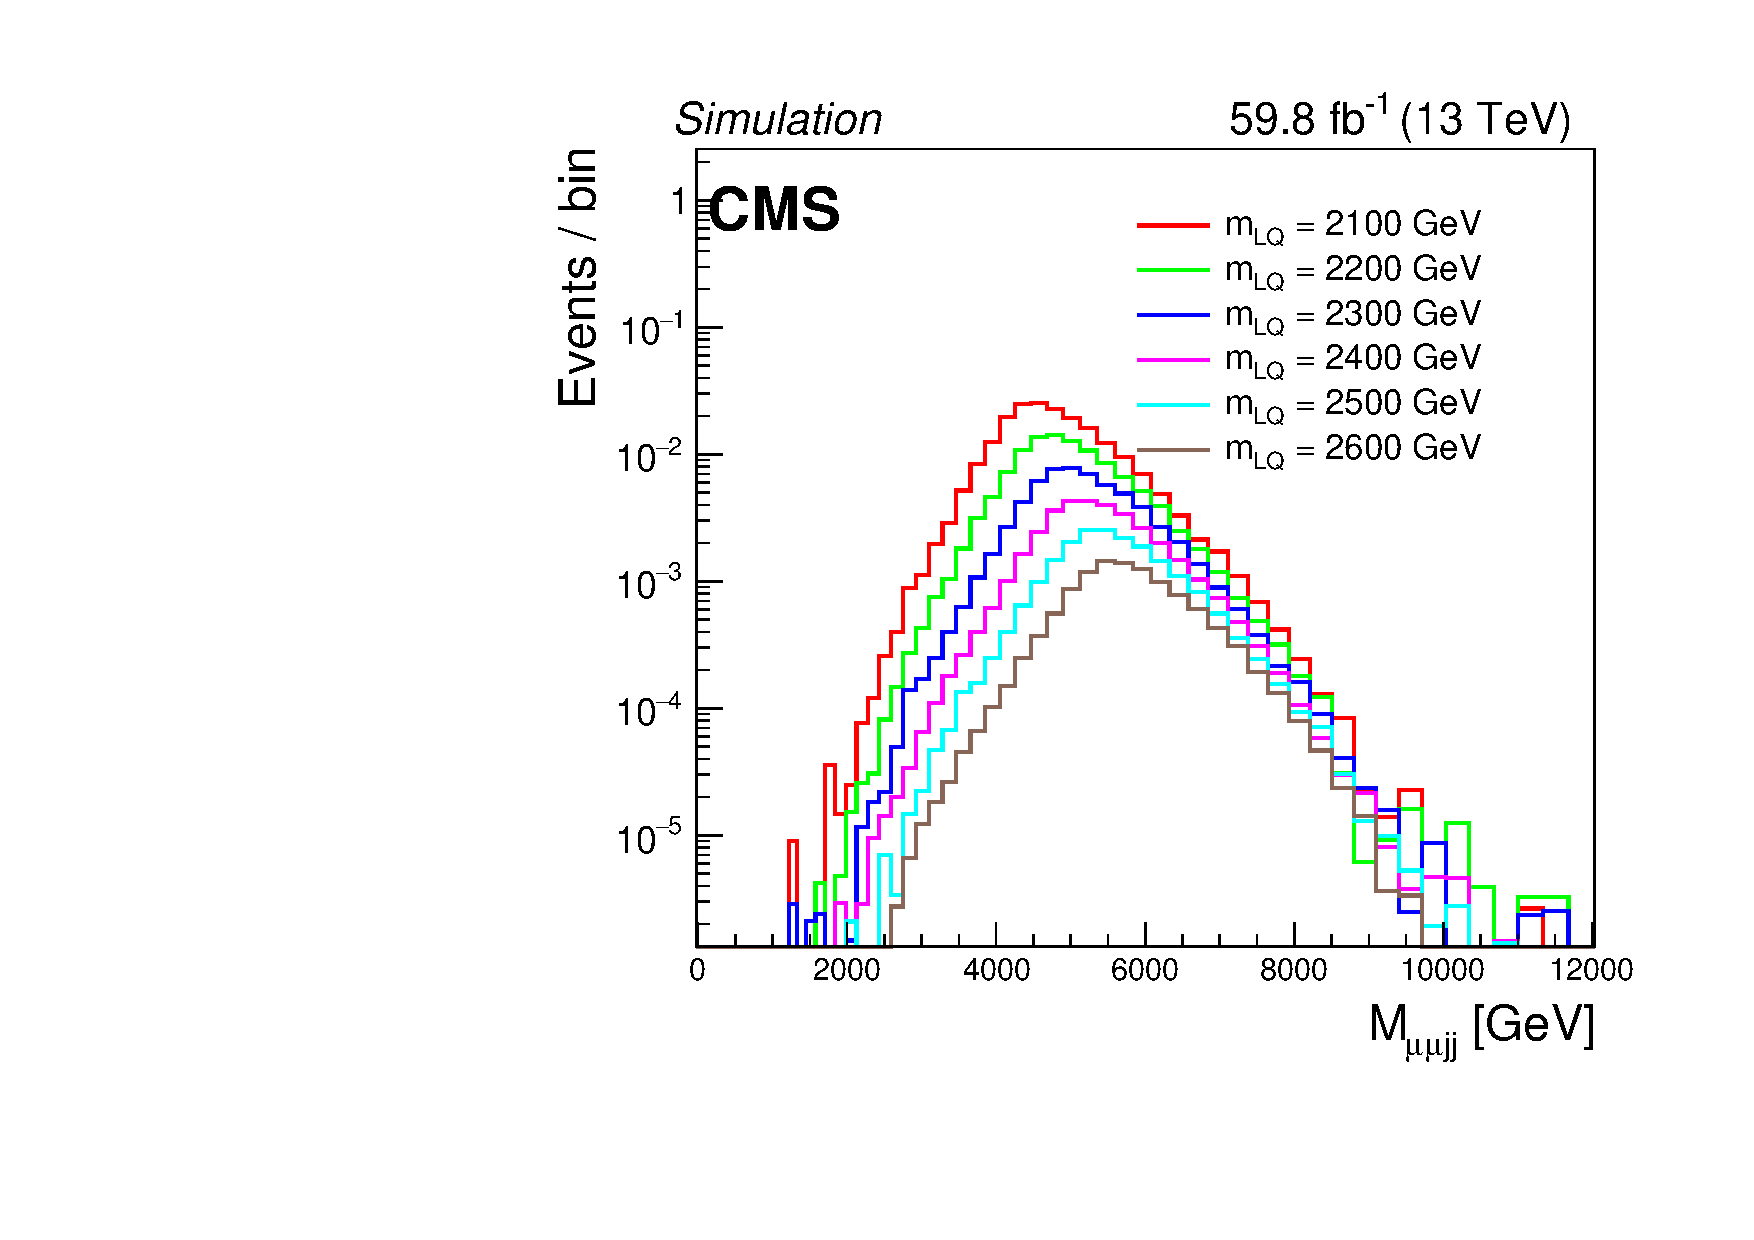
\includegraphics[width=.32\textwidth]{Images/Analysis/SignalMassStudy/2018/Mujbj_M2100_to_M2600.pdf}}
    {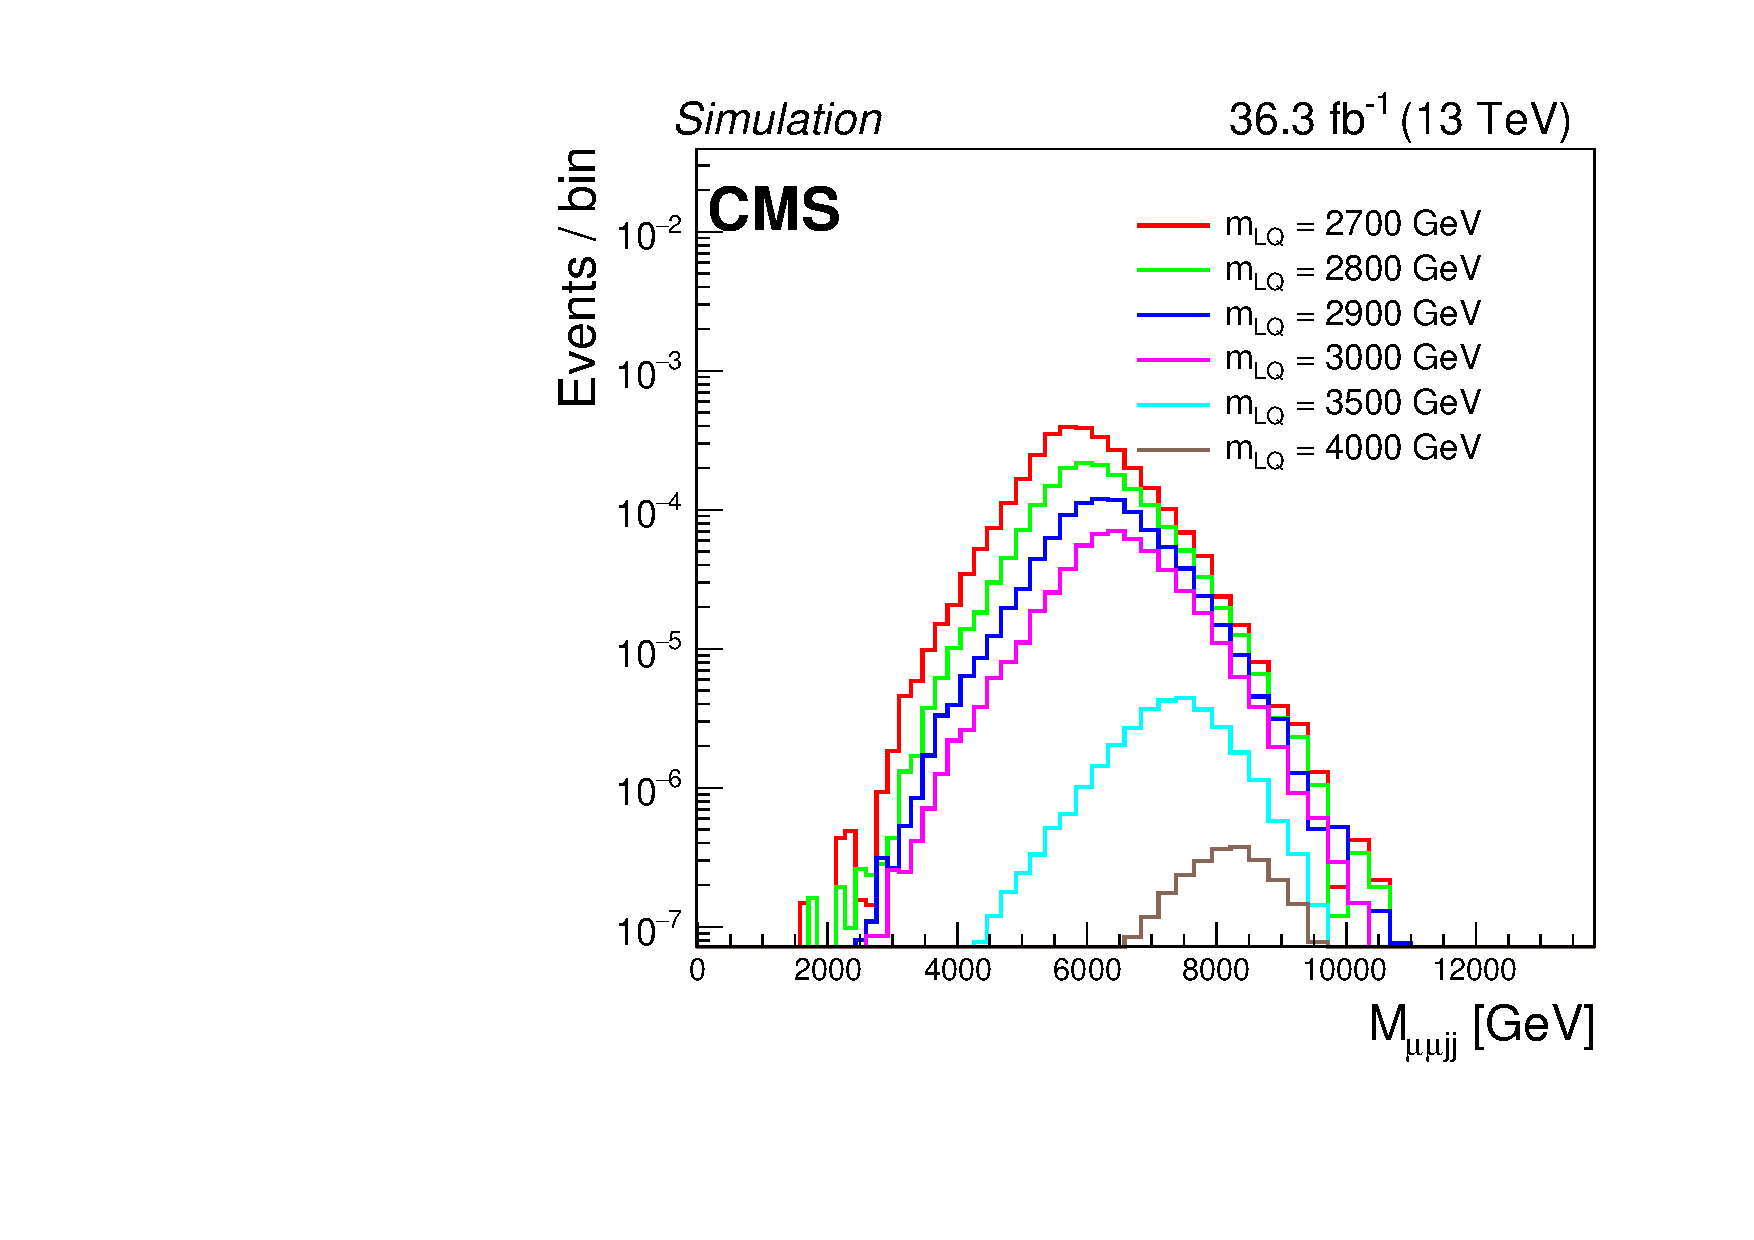
\includegraphics[width=.32\textwidth]{Images/Analysis/SignalMassStudy/2016/Mujbj_M2700_to_M4000.pdf}}
    {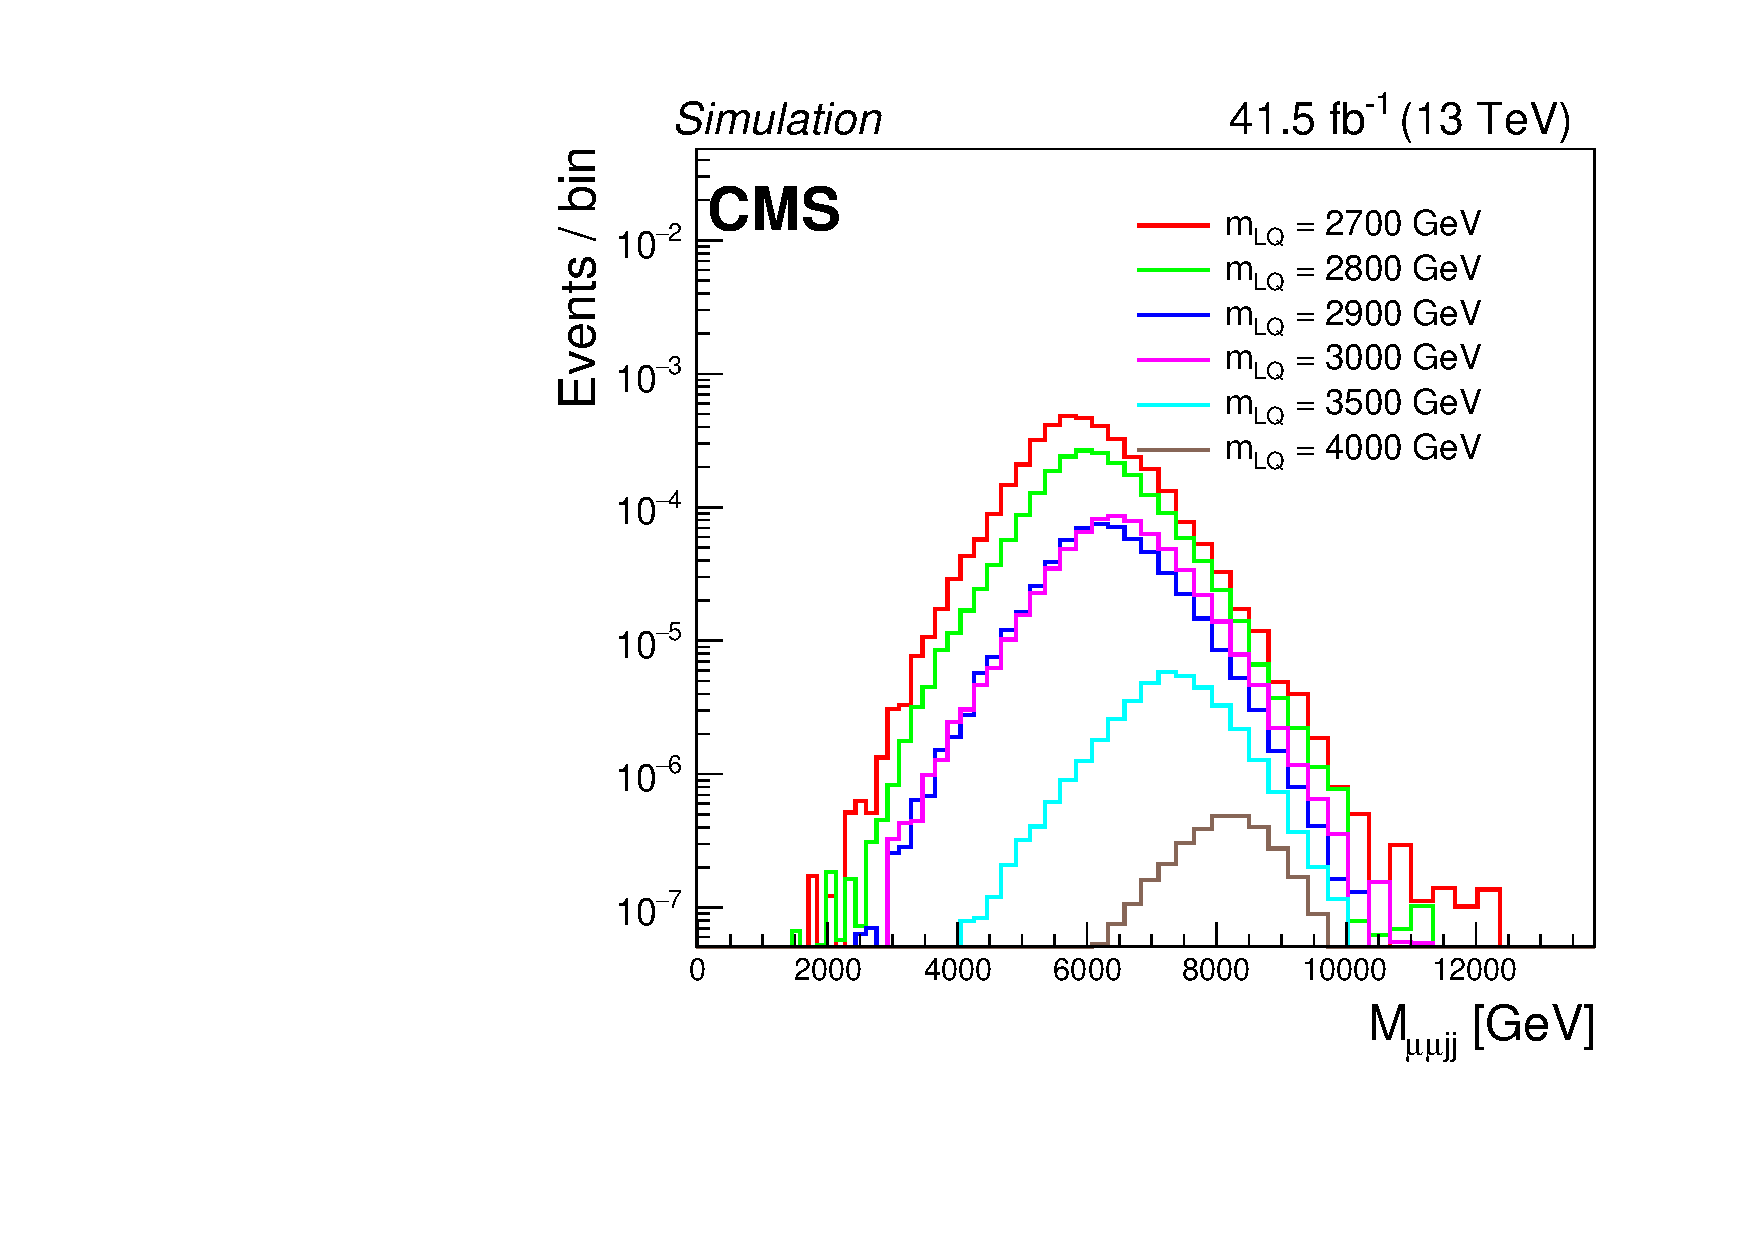
\includegraphics[width=.32\textwidth]{Images/Analysis/SignalMassStudy/2017/Mujbj_M2700_to_M4000.pdf}}
    {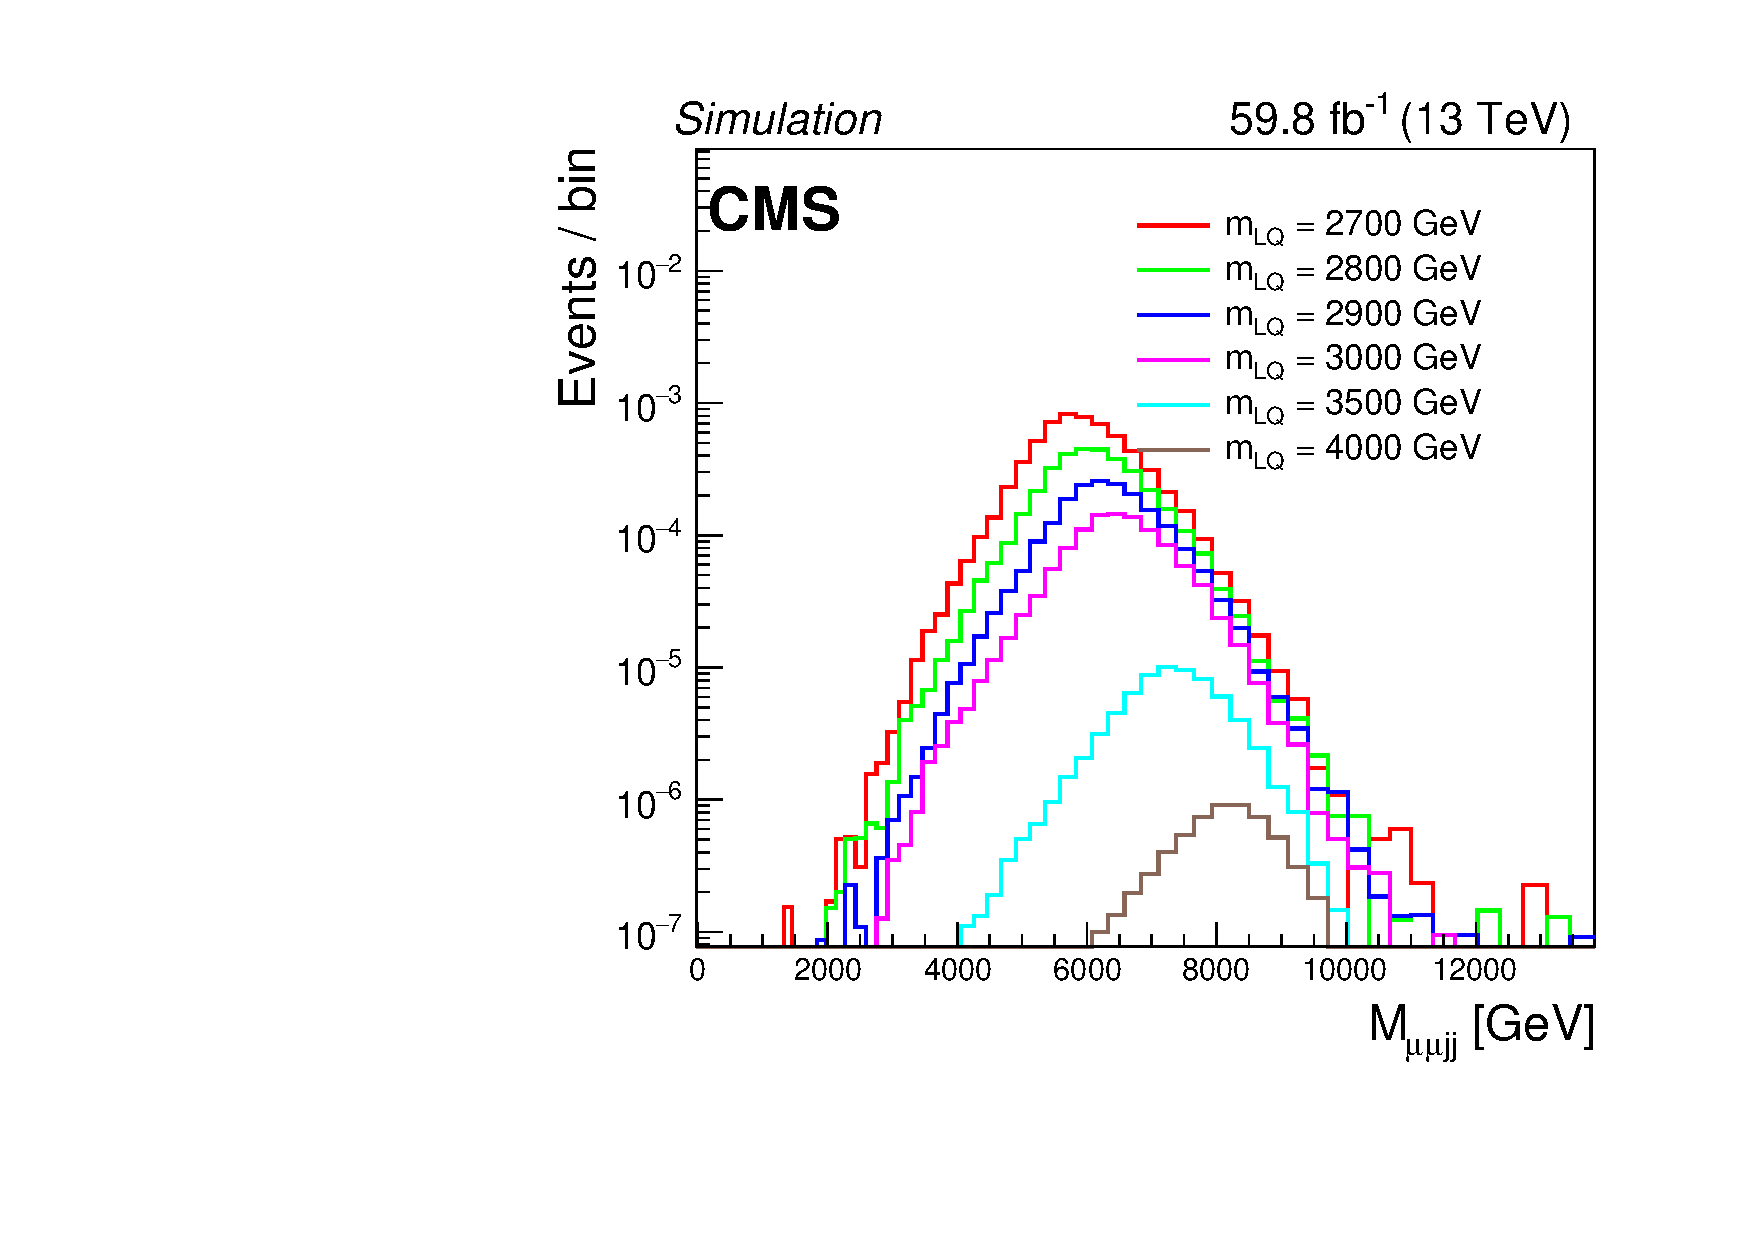
\includegraphics[width=.32\textwidth]{Images/Analysis/SignalMassStudy/2018/Mujbj_M2700_to_M4000.pdf}}
    \caption{The preselection-level \Muujj distributions of simulated leptoquark pair samples for the data-taking periods 2016 (left), 2017 (middle), and 2018 (right). For clarity, each plot overlays the distributions corresponding to a set of six leptoquark masses: \SI{2100}{} to \SI{2600}{GeV} (top) and \SI{2700}{} to \SI{4000}{GeV} (bottom).}
    \label{figapp:lqsim2}
\end{figure}